\newpage

\chapter{Мотивация и постановка задачи}
\label{ch:chapter_1}

\section{Диаграммы связей}
\label{sec:mindmaps}
Диаграмма связей представляет собой древовидную структуру, пример на
рис.~\ref{pic:mindmap}.

\begin{figure}[h!]
  \centering 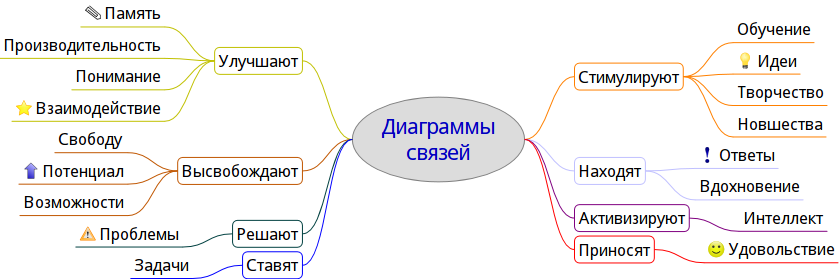
\includegraphics[width=1\linewidth]{mindmap}
  \caption{Пример диаграммы связей}
  \label{pic:mindmap}
\end{figure}

Диаграмма связей состоит из узлов и соединительных линий между ними. Зачастую,
информация, структурированная подобным образом, воспринимается лучше, чем
обычный текст. Оформление диаграммы связей играет большую роль в её восприятии и
осознании. Множество ключевых идей может быть выделено среди всех остальных,
используя атрибуты узла или дуг. К примеру, выделить схожие идеи одинаковым
цветом или поставить пиктограмму напротив некоторых из них. Также существует
возможность скрыть некоторые узлы, чтобы сконцентрироваться на требуемой части
диаграммы. Чем больше доступных способов оформления, тем более точно могут быть
выражены ассоциативные связи между узлами, что в свою очередь способствует
процессу ассоциативного мышления.


\section{Описание проекта HiveMind}
\label{sec:project_summary}
Главной целью проекта HiveMind является разработка редактора диаграмм связей,
удовлетворяющего следующим требованиям: кросс-платформенность, богатая
функциональность, поддержка функций совместного редактирования.

Мобильные устройства получили большое распространение в современном мире.
Зачастую, приложение, предназначенное для на настольного компьютера, неудобно
или невозможно использовать на мобильных устройствах. Специфика мобильных
устройств, по сравнению с настольными компьютерами, заключается в малом
разрешении экрана и наличии альтернативных средств ввода. Данные различия
требуют абсолютно иного подхода к построению пользовательских интерфейсов на
мобильных устройствах. Множество людей пользуются мобильными устройствами вне
дома и настольными компьютерами у себя дома. Пользователь использует множество
операционных систем: Windows, Linux, MacOS на настольных компьютерах и Maemo,
Android, MeeGo на мобильных устройствах. Пользователь нуждается в том, чтобы
необходимое ему приложение было доступно под все виды используемых им платформ.
Данный факт ставит перед разработчиками приложений абсолютно новую задачу  ''---
разработка кросс-платформенных приложений с интерфейсом оптимизированным под
настольные и мобильные платформы \cite{hivemind-8th-fruct}.

Существует множество приложений для редактирования диаграмм связей (FreeMind,
Xmind, Vym, iMindMap и т.д.) и веб-сервисов в сети Интернет (MindMeister,
Mind42, Mindomo и т.д.). Данные редакторы были рассмотрены на предмет
соответствия следующим требованиям:
\begin{itemize}
\item кросс-платформенность;
\item широкий функционал;
\item поддержка функций совместного редактирования;
\item бесплатность.
\end{itemize}
На текущий момент, не существует редакторов диаграмм связей, удовлетворяющих
вышеперечисленным требованиям \cite{hivemind-8th-fruct}. Поэтому было принято
решение о разработке соответствующего приложения.

В настоящее время, приложение HiveMind обладает следующими возможностями:
\begin{itemize}
\item чтение и запись файлов в формате FreeMind;
\item отображение диаграмм связей и навигация по ним;
\item интерфейс, оптимизированный для настольных и мобильных устройств;
\item интернационализация;
\item кросс-платформенность (Поддержка Windows, Linux, Maemo, MeeGo);
\item использование клавиатуры и сенсорного дисплея.
\end{itemize}


\section{Используемый инструментарий}
\label{sec:toolkit}
Приложение HiveMind написано на языке программирования Python с использованием
библиотеки Qt.

Qt "--- Кросс-платформенный фреймворк, используемый для разработки ПО
~\cite{qt4}. Широко используется для построения приложений с графическим
интерфейсом, так и с интерфейсом командной оболочки. Изначально, библиотека Qt,
написана на C++, но может быть использована на других язык программирования,
используя соответствующие <<привязки>>. Данная библиотека обладает широкой
функциональностью и имеет множество модулей, обеспечивающий работу с 3D
графикой, веб и мультимедиа контентом, базами данных, сетью и т.д.

Python "--- Интерпретируемый, высокоуровневый язык программирования общего
назначения ~\cite{python}. Он нацелен на быстроту написания и легкую читаемость
кода, обладает понятным и минималистичным синтаксисом. Python имеет поддержку
следующих парадигм программирования: объектно-ориентированное, функциональное,
процедурное, аспектно-ориентированное, императивное. Из особенностей языка
следует отметить динамическую типизацию, автоматическое управление памятью,
полную поддержку метапрограммирования и механизм обработки исключений. С данным
языком поставляется большая и многофункциональная библиотека, являющаяся одной
из сильных сторон языка. Помимо всего прочего, язык поддерживает написание
внешних модулей на языках C и C++. Интерпретаторы языка Python доступны под
множеством операционных систем.

PyQt "--- набор <<привязок>> фреймворка Qt для языка программирования Python.
PyQt реализует более чем 440 классов и 6000 методов библиотеки Qt, включающих в
себя классы для построения графического интерфейса пользователя, работы с БД,
сетью, XML, SVG и т.д. PyQt лицензирован под двумя лицензиями: GPL и
коммерческой, что позволяет бесплатно использовать его в проектах с открытым
исходным кодом.

Приложение HiveMind является кросс-платформенным и работает под следующими
операционными системами: Windows, Linux, Meego, Maemo. ОС MeeGo ориентирована на
устройства на базе нетбуков, планшетов и ноутбуков, ОС Maemo на мобильные
устройства, в то время как Linux и Windows на настольные компьютеры и ноутбуки.
Каждые из целевых платформ имеют разные форм-факторы, устройства ввода и
соединение с сетью.


\section{Концепция совместного редактирования диаграмм связей}
\label{sec:collaborative_mindmapping}
В общем виде, процесс совместного редактирования диаграмм должен выглядеть
следующим образом. Пользователь, с установленным приложением HiveMind, в любой
момент может открыть доступ к своей диаграмме связей. Другой пользователь
подключается к диаграмме связей данного человека, автоматически получает её
актуальную копию и оба пользователя начинают совместное редактирование
диаграммы. Количество пользователей, участвующих в процессе совместного
редактирования, должно быть неограничено. Пользователь, открывший доступ к
карте, должен иметь возможность изменения прав доступа участников к процессу
совместного взаимодействия. Далее перечисляются возможные сценарии использования
функций совместного редактирования диаграмм связей.

Пользователь создаёт диаграмму связей и начинает её редактирование, используя
мобильное устройство, ноутбук или персональный компьютер. В процессе
редактирования, пользователь решает показать свою работу другу (к примеру, для
получения помощи). Пользователь открывает доступ к своей диаграмме. В данном
случае, устройство, на котором запущено приложение, начинает работать как
сервис, доступный из локальной сети или интернет. Другой пользователь
подключается к диаграмме связей и автоматически получает актуальную копию
диаграммы. Далее оба пользователя начинают совместное редактирование диаграммы.
Количество взаимодействующих участников неограниченно, поэтому другие
пользователи также могут участвовать в совместной работе. Изменения, совершаемые
каждым из участников, незамедлительно посылаются остальным участникам.

Следующий сценарий использования совместного редактирования диаграмм связей
может быть полезен при представлении докладов. К примеру, докладчик имеет
дополнительные материалы, такие как: план презентации, краткий обзор речи
выступления или ссылки на дополнительные ресурсы. Докладчик оформляет данные
материалы в виде диаграммы связей и открывает к ней доступ. Используя HiveMind
на мобильных устройствах или нетбуках, cлушатели подключаются к диаграмме
связей, выложенной докладчиком. Таким образом, слушатели получают материалы
подготовленные докладчиком, а также получают уведомления обо всех изменениях,
сделанных докладчиком в процессе выступления.

Диаграмма связей может содержать материалы для дискуссии в реальном времени. В
данном случае, она может быть использована, как лекционная доска с иерархической
структурой, на которую каждый участник может заносить свои идеи, комментарии или
мнения. Главное преимущество такого рода обсуждений, с использованием HiveMind,
то, что данные имеют иерархическую структуру и доставляются всем участникам
почти мгновенно.

Пользователь может хранит на диаграмме связей свою личную информацию, поэтому,
открывая доступ к диаграмме, он должен иметь возможность ограничить круг
лиц, имеющих доступ к диаграмме. Также необходимо контролировать права доступа
участников на редактирование диаграммы. К примеру, при выступлении двух
докладчиков перед аудиторией, необходимо разрешить редактирование диаграммы
только выступающим и запретить всем остальным.


\section{Постановка задачи}
\label{sec:problem_statement}
Задача заключается в том, чтобы реализовать возможность совместного
редактирования диаграмм связей в проекте HiveMind.

Существует множество способов установить сетевое взаимодействие между
приложениями, начиная от низкоуровневой обработки пакетов на уровне стека
TCP/IP, заканчивая использованием высокоуровневых объектно-ориентированных
библиотек для протоколов прикладного уровня. С точки зрения реализации,
использование низкоуровневых средств чрезмерно затратно и было решено
использовать высокоуровневую технологию. На сегодняшний день доступно огромное
количество подобных технологий и встаёт задача об её выборе.

Приложение HiveMind нацелено на использование на мобильных и
настольных платформах. Данные типы платформ различаются способом соединения с
сетью Интернет и набором библиотек, доступных для использования. Из этих фактов
вытекают несколько задач:
\begin{itemize}
\item произвести сравнительный анализ способов соединения с сетью Интернет для
разных платформ;
\item выбрать технологию промежуточного слоя на основе проведенного анализа;
\item выбрать библиотеку для работы с технологией, доступную на всех целевых
платформах.
\end{itemize}

Следующим шагом является разработка сетевой архитектуры. Cетевая подсистема
должна быть построена на основе существующего приложения, имеющего большую
кодовую базу (более 10000 строк кода), богатую функциональность и наличие
множества архитектурных решений. Сетевая подсистема должна удовлетворять
следующим требованиям:
\begin{itemize}
\item реализация виде отдельных модулей, слабо связанных с существующим
приложением;
\item гибкая архитектура, возможность добавления новых типов передаваемых
данных;
\item потенциально неограниченное количество участников;
\item наличие механизма обнаружения потери соединения и переподключения;
\item минимальные задержки при передачи данных.
\end{itemize}
Разработанное приложение должно иметь функциональность, обеспечивающую
взаимодействие по всем сценариям перечисленным в пункте
\ref{sec:collaborative_mindmapping}.


